\subsection{Zielsetzung}

Das Hauptziel des Capacitor-BrowserView Plugins ist die Entwicklung eines Plugins für Capacitor, welches Entwicklern ermöglicht, zusätzliche Webbrowser-Fenster (WebViews) innerhalb einer Capacitor Anwendung zu erstellen und zu steuern.
Diese Fenster können zum Anzeigen und Manipulieren von zusätzlichen Webinhalten verwendet werden.
Dies ist praktisch, um externe Inhalte dynamisch anzuzeigen und von der Capacitor-Anwendung zu isolieren.

Darüber hinaus soll eine optional zu aktivierende Kommunikation zwischen geladenen Webinhalten und der Capacitor Anwendung ermöglicht werden.
Dies ist sinnvoll, wenn ein vertrauenswürdiger externer Inhalt geladen wird, der nicht vollständig isoliert werden soll, da ein Datenaustausch mit diesem Inhalt und der Capacitor Anwendung benötigt wird.

Das Plugin soll ohne zusätzlichen Aufwand sowohl in Mobile"=Anwendungen als auch in Desktop"=Anwendungen eingesetzt werden können.

\begin{figure}[H]
    \centering
    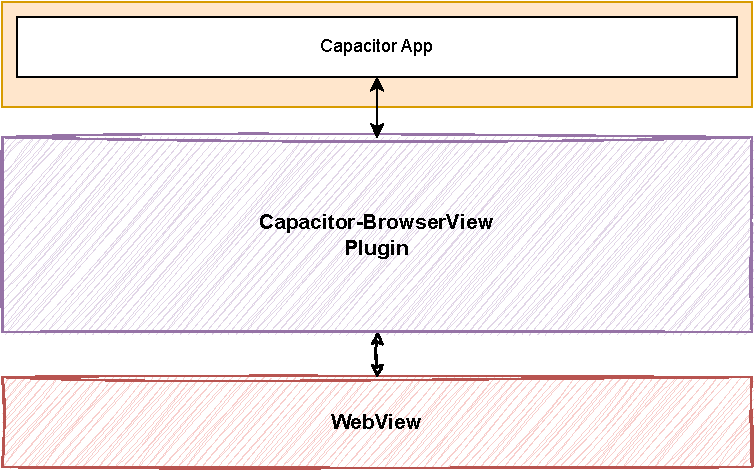
\includegraphics[width=0.8\textwidth]{assets/03_Capacitor-BrowserView/01_Zielsetzung.drawio.pdf}
    \caption[Capacitor-BrowserView / Zielsetzung]{Zielsetzung des Capacitor-BrowserView Plugins}
\end{figure}

Die vom Plugin implementierten Webbrowser-Fenster bzw.\ unter Android und iOS genannten WebViews werden im Plugin als BrowserViews bezeichnet, um die Ähnlichkeit mit den bereits in Electron existierenden BrowserViews zu verdeutlichen.
\cite{android:api, ios:api, electron:docs}

\begin{note}
    Die offizielle Entwicklungsumgebung für iOS, Xcode, ist ausschließlich für macOS verfügbar.~\cite{xcode:support}
    Da während der Entwicklung nur Windows- und Linux-Geräte zur Verfügung standen, war das Implementieren und Testen des Plugins für iOS nicht möglich.
\end{note}
